\section{Introduction}

\M I was reflecting upon my notes, and realized how much I enjoyed
taking courses from Dr Albert Schwarz while at UC Davis. I also wanted
to review supermathematics.

\M
We will study supermathematics by means of puzzles and exercises.
``Puzzles'' are more ``longterm'' questions to ponder, which we may
answer in future sections. ``Exercises'' are questions I want you to
answer as you read them. Or, if we think of this article as a road
trip, the ``puzzles'' are ``mileage signs'' and the ``exercises'' are the
next offramp.

\begin{figure}[h]
  \centering
  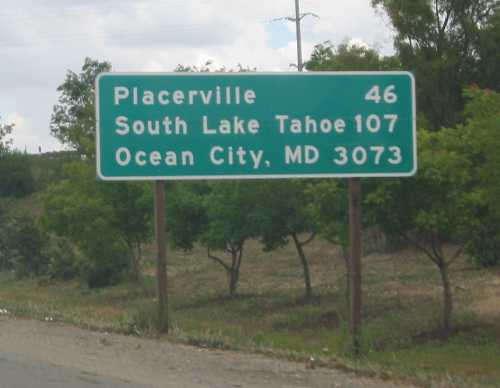
\includegraphics[width=7.55cm]{img/ocean-city.JPG}
  \caption[Mileage sign]{Every student at UC Davis recognizes this mileage sign on the
    Interstate-80 East. Note: 3073 miles is about 4945.5 kilometers. Taken from the DavisWiki, photo by Miriam Kaufman.\footnotemark}
\end{figure}
\footnotetext{See \url{https://localwiki.org/davis/Interstate_80} and \url{https://localwiki.org/davis/Interstate_80/_files/OceanCity.JPG/_info/}}
